The business canvas gives an overview of Valcon's business.
Based on our analysis we have the following understanding of Valcon's canvas.
\begin{figure}[!htp]
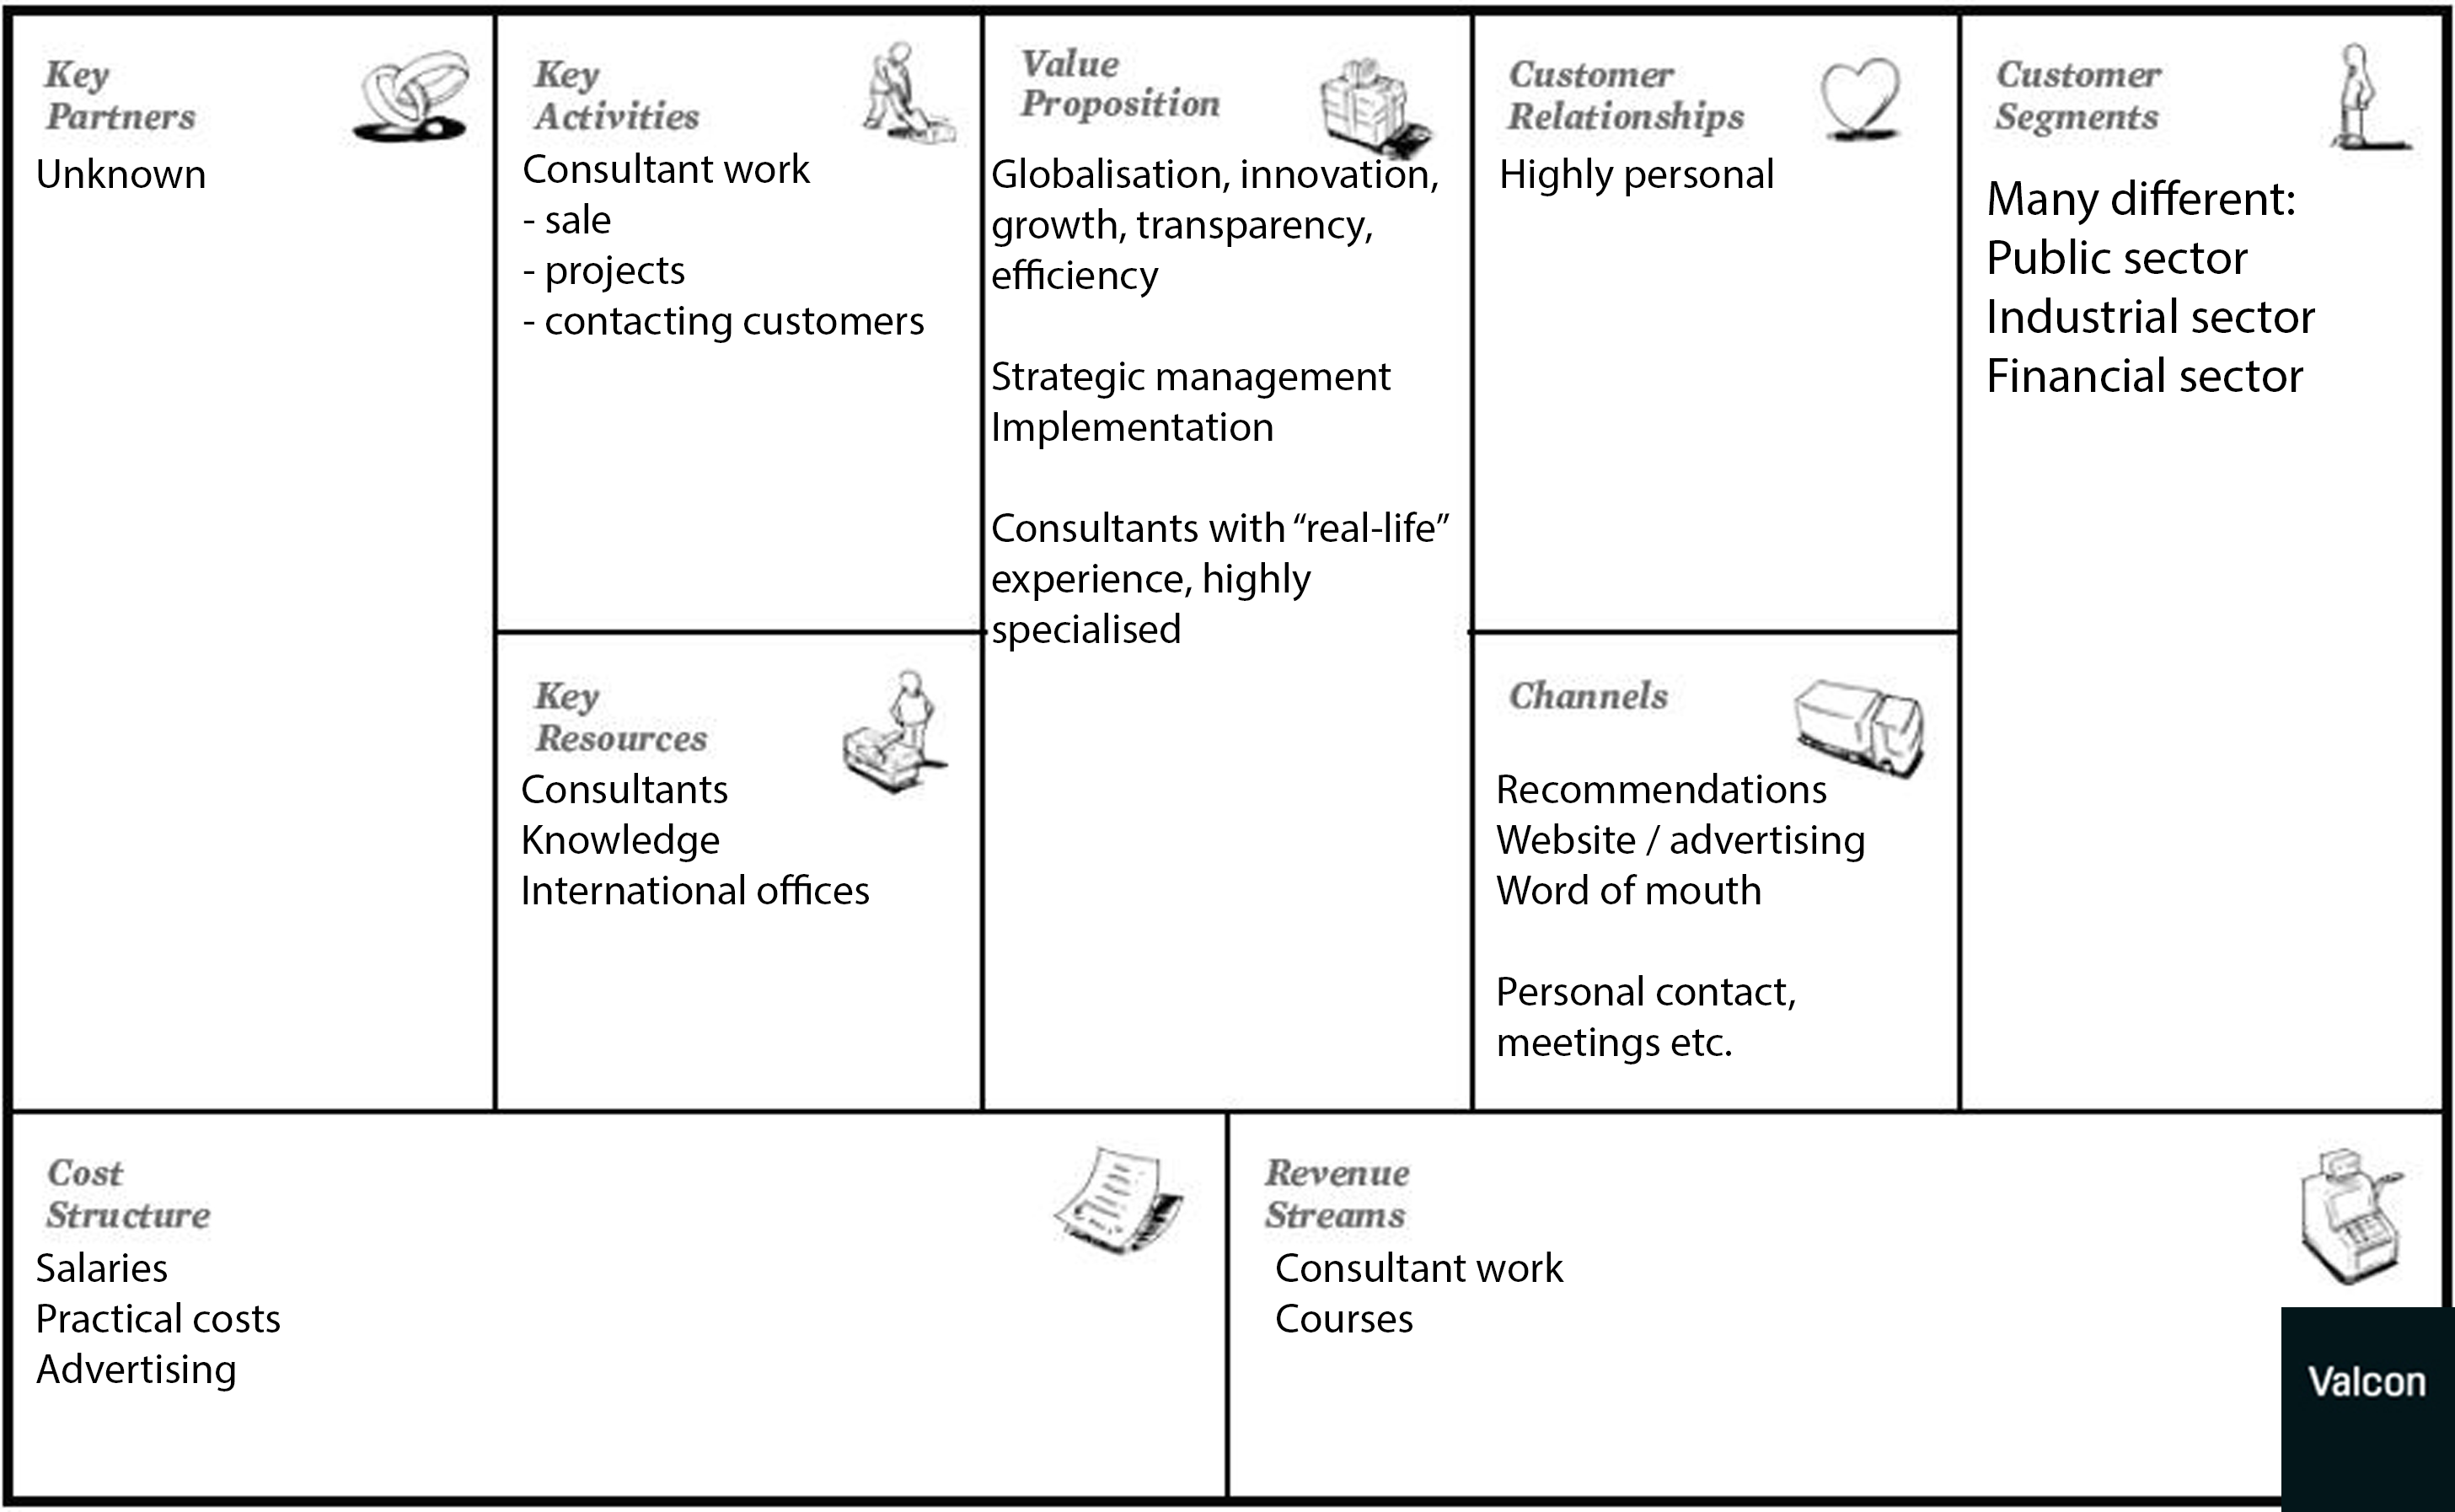
\includegraphics[width=\textwidth]{inline/business-model-canvas.png}
\caption{Valcon's business canvas.}
\label{fig:canvas}
\end{figure}

The Business Canvas gives an overview of Valcon as a whole. In relation to the problem it is important to note that the consultants are key resources for Valcon's business, as they are the ones who generate revenue.
As such it is important that they are able to perform their work effectively as soon as they start working at Valcon. It gives us a good understanding of why the company might value the consultants' time highly. (Sources: Initial meeting with Danni (appendix \ref{app:danni_initiation}), Valcon's homepage. Approved by Danni during inline conclusion meeting (appendix \ref{app:danni_inline}).) (See appendix \ref{app:canvas}.)

We have chosen not to do a canvas for OMT because \todo{Why no OMT canvas?}